\chapter{Formatting instructions}
\label{ch:formatting}

One thing you'll notice is that the title gets converted to all caps automatically by the class file, in agreement with the NJIT style guidelines!

\section{\BibTeX\ Style}

The default bibliography format is set in the file \texttt{dmsthesis.cls} by the line \verb+\bibliographystyle{acm}+. There should be no reason to change it.

Finally, let's try a few citations \cite{ALBERTSETAL:1994,FERSHT:1985,FISCHER:1987a,KAUFFMAN:1969,MR1191182,MR1617060}. 

\section{Symbols}
\opensymdef
\newsym[Energy]{symE}{E}
\newsym[Mass]{symm}{m}
\newsym[Speed of light]{symc}{c}
\closesymdef

Now I can use the inline symbol: \symE\ defined in \texttt{symbols.tex} \[\symE=\symm \symc^2\] where
\symE\ is the energy \ldots

\section{Example Section With Figure}

NJIT's style guide says that the figure caption should be left justified. The text in the caption should be repeated verbatim in the List of Figures. Both of these are taken care of automatically by the template.

\begin{figure}[htbp]
\centering

\includegraphics[width=4.5in]{msgcube}
\caption{This is the logo of MSG, the Mathematical Science Group. Do not use the alternate caption feature in \LaTeX. The entire caption must be reproduced in the list of figures.}
\label{fig:1}
\end{figure}


We can also make subfigures. We can reference them separately like Figure~\ref{fig:first}, Figure~\ref{fig:second} and together like Figure~\ref{fig:doublefigure}.
\begin{figure}
\centering
\begin{subfigure}{0.4\textwidth}
    
\includegraphics[width=\textwidth]{FancyA.jpg}
    \caption{A fancy letter A.}
    \label{fig:first}
\end{subfigure}
\hfill
\begin{subfigure}{0.4\textwidth}
    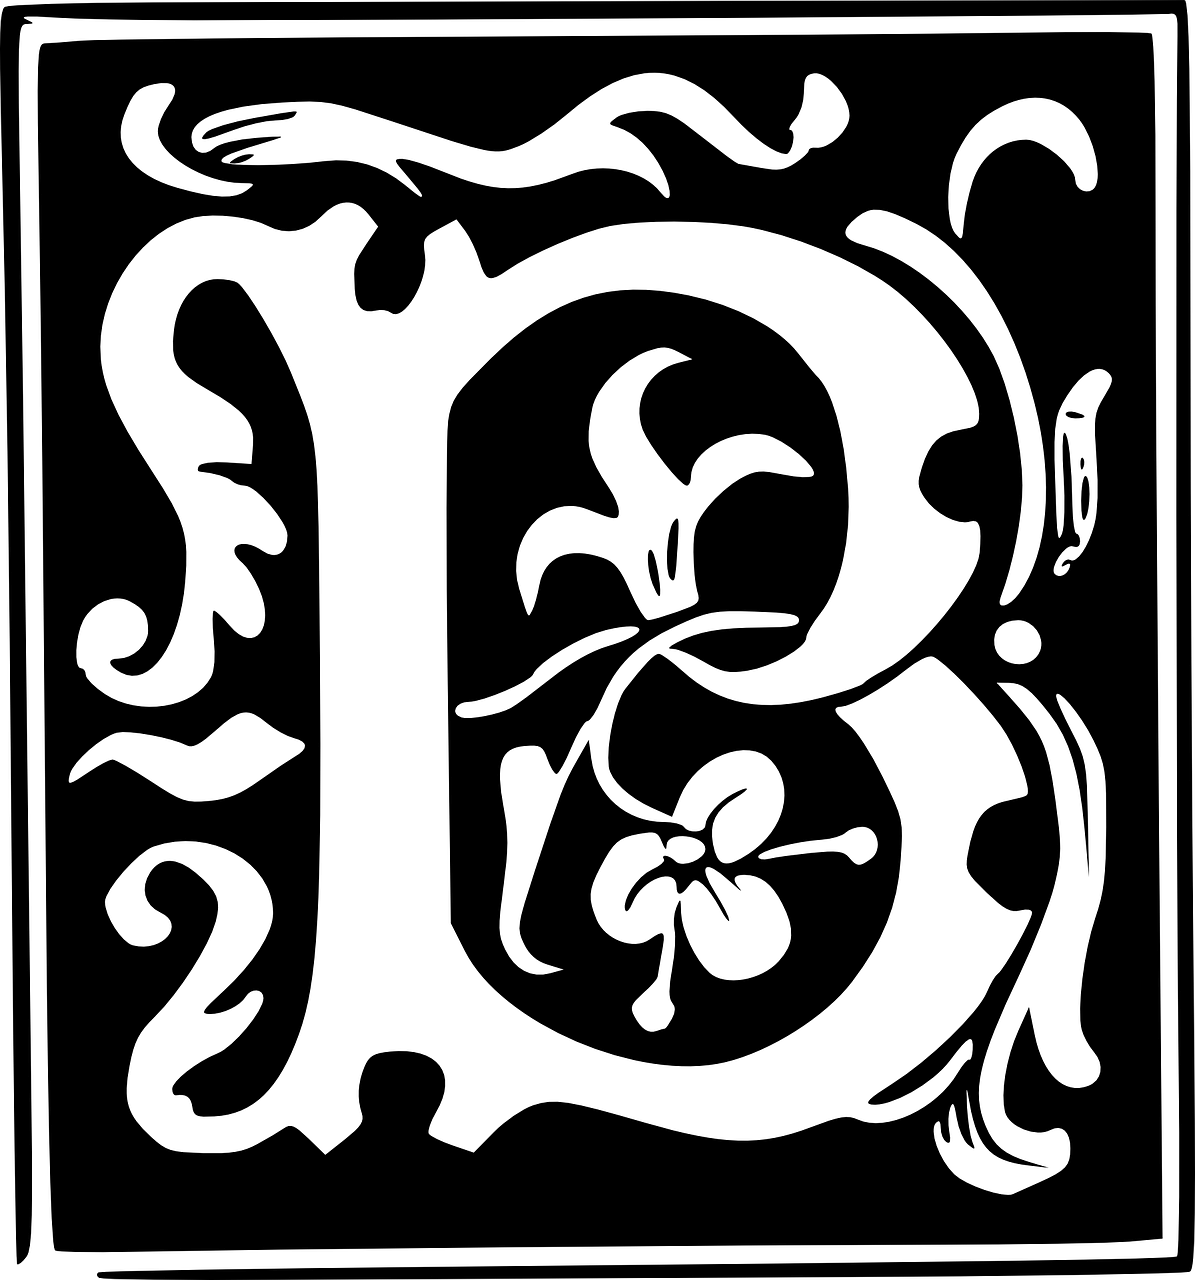
\includegraphics[width=\textwidth]{FancyB.png}
    \caption{A fancy letter B.}
    \label{fig:second}
\end{subfigure}
\caption{A figure with two subfigures.}
\label{fig:doublefigure}
\end{figure}

\newpage
\subsection{Example Subsection With Table}

Here is an example of a table. Note that caption of the table is written with initial capitals, like  a Section or Subsection, and note that it doesn't end with a period as figure caption. Also, the caption is above the table.  You can achieve this by put \verb#\caption{}# command all the way on the top.  You might need to forcibly add space between the text and the table so that it doesn't appear too close to the text.  View the file \texttt{table.tex} for details of the table.
\vspace{4mm}

\renewcommand{\baselinestretch}{0.8}
\newcommand{\PreserveBackslash}[1]{\let\temp=\\#1\let\\=\temp} 
\let\PBS=\PreserveBackslash
\begin{table}[htbp]
\centering
\begin{minipage}{0.89\textwidth}
\caption[Major Differences Between Neural Networks and Cell Signaling Networks]{Major Differences Between Neural Networks and Cell Signaling Networks\protect\footnote{You can also have footnote in table as in figure.}}
\vskip .25in
\label{table:NN_DIFF}

  \footnotesize
    \begin{tabular}
	{|p{0.04 \textwidth}
	|p{0.15 \textwidth}
	|p{ 0.35 \textwidth}
	|p{ 0.35 \textwidth}|} \hline
	\rule{0pt}{1pt} & & & \\
	\strut & 
		\PBS\raggedright{\em Salient features of networks} &
		\PBS\raggedright{\em Neural Networks} &
		\PBS \raggedright{\em Cell Signaling Networks}\\
	\rule{0pt}{1pt}& & & \\ \hline
	\rule{0pt}{1pt}& & & \\
	\strut (i)  & 
		\PBS\raggedright{nodes} & 
		\PBS\raggedright{all nodes typically identical} &
		\PBS\raggedright{nodes are not all equivalent in performance} \\
	\rule{0pt}{1pt}& & & \\ \hline
	\rule{0pt}{1pt}& & & \\
	\strut (ii) & 
		\PBS\raggedright{structure} &
		\PBS\raggedright{typically layered with feed-forward connections only} &
		\PBS\raggedright{regulatory signals often give rise to feedback connections resulting in cycles} \\
	\rule{0pt}{1pt}& & & \\ \hline
	\rule{0pt}{1pt}& & & \\
	\strut (iii) & 
		\PBS\raggedright{connectivity} & 
		\PBS\raggedright{highly connected} &
		\PBS\raggedright{more sparsely connected} \\
	\rule{0pt}{1pt}& & & \\ \hline
	\rule{0pt}{1pt}& & & \\
	\strut (iv) &  
		\PBS\raggedright{learning rule} &
		\PBS\raggedright{connectivity altered to perform a single function e.g.,~via a back-propagation algorithm} &
		\PBS\raggedright{cells must be able to respond to multiple stimuli effectively;changes typically occur via evolutionary processes} \\

	\rule{0pt}{1pt}& & & \\ \hline
    \end{tabular}
\\
\end{minipage}
\end{table}
\renewcommand{\baselinestretch}{1.65}



\begin{equation}
x^2+1
\end{equation}

